\documentclass{article}  
\usepackage[a4paper]{geometry}
\usepackage{fancyhdr}
\pagestyle{fancy}
\lhead{Baumdiagramme}
\rhead{August 2025}
\usepackage{tikz} 
\begin{document} 
\section{Baumdiagramme}
\begin{minipage}{\dimexpr\linewidth-5cm} 
 Ein Baumdiagramm ist ein Diagramm, welches von einem Ausgangspunkt aus die direkten Folgen verbindet, diese können wiederum ein eigener Ausgangspunkt, oder ein Endergebnis sein. Auf den Verbindungslinien, steht die Wahrscheinlichkeit, dass basierend auf dem Ausgangspunkt ein bestimmtes Ereigniss eintritt. Die Wahrscheinlichkeit, dass ein Endergebnis eintritt, ist das Produkt aller Wahrscheinlichkeiten der Pfade, welche dazu geführt hatten, dass dieses eintritt.
\end{minipage}
\hfill
\begin{minipage}{5cm}
 \center
 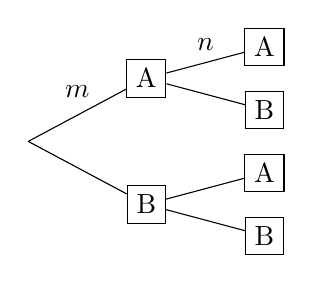
\begin{tikzpicture}
    \node[draw] (a) at (1.5,0.8) {A};
    \node[draw] (b) at (1.5,-0.8) {B};
 
    \node[draw] (aa) at (3,1.2) {A};
    \node[draw] (ab) at (3,0.4) {B};
 
    \node[draw] (ba) at (3,-0.4) {A};
    \node[draw] (bb) at (3,-1.2) {B};
    \draw (0, 0) -- (a) node[midway, above, yshift=3pt] {$m$}; 
    \draw (0, 0) -- (b);
 
    \draw (a) -- (aa) node[midway, above, yshift=1pt] {$n$};  
    \draw (a) -- (ab);  
    \draw (b) -- (ba);  
    \draw (b) -- (bb); 
 \end{tikzpicture} 
\end{minipage}
\vspace{-0.35em} \newline
Das Beispielbaumdiagramm, rechts, zeigt, dass vom Ausgangspunkt aus die Chance, dass A eintritt, bei $m$ liegt. Ist A bereits einmal eingetreten, ist liegt die Wahrscheinlichkeit dass es erneut eintritt bei $n$. Somit ist $P(A, A) = m \cdot n$ 
 
 
\end{document}